\documentclass[11pt]{article}

% PACKAGES
\usepackage{amsmath}
\usepackage{amssymb}
\usepackage{graphicx}
\usepackage[margin=1in]{geometry}
\usepackage{hyperref}
\usepackage{tikz}
\usetikzlibrary{decorations.markings}
\usetikzlibrary{arrows.meta}

% DOCUMENT INFO
\title{Concise Notes and Problems on Electromagnetic Induction}
\author{}
\date{\today}

\begin{document}

\maketitle
\tableofcontents
\newpage

\section{Notes on Electromagnetic Induction (EMI)}

\subsection{What is Electromagnetic Induction? \_a}
Electromagnetic induction is the process of generating an electromotive force (EMF), which is essentially a voltage, in a conductor by changing the magnetic field around it. A changing magnetic field creates an electric field. This discovery by Michael Faraday is the principle behind electric generators, transformers, and induction cooktops.

\subsection{Magnetic Flux ($\Phi_B$)}
Magnetic flux is a measure of the total magnetic field lines passing through a given area.

\begin{itemize}
    \item \textbf{Equation:} For a uniform magnetic field $\vec{B}$ passing through a flat area $\vec{A}$, the flux is:
    $$ \Phi_B = \vec{B} \cdot \vec{A} = BA\cos\theta $$
    where $\theta$ is the angle between the magnetic field $\vec{B}$ and the normal to the area, $\vec{A}$.
    
    \begin{center}
    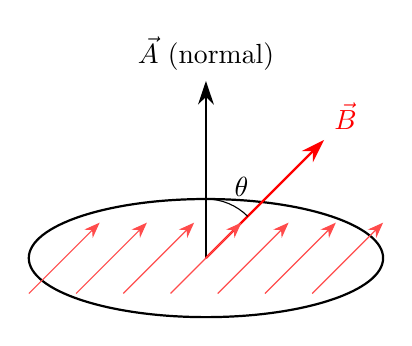
\begin{tikzpicture}[scale=1.5]
        % Draw the loop
        \draw[thick] (0,0) ellipse (1.5cm and 0.5cm);
        % Draw the normal vector
        \draw[-{Stealth[length=3mm, width=2mm]}, thick] (0,0) -- (0,1.5) node[above] {$\vec{A}$ (normal)};
        % Draw the B-field vector
        \draw[-{Stealth[length=3mm, width=2mm]}, thick, red] (0,0) -- (1,1) node[above right] {$\vec{B}$};
        % Draw the angle
        \draw (0,0.5) arc (90:45:0.5cm);
        \node at (0.3,0.6) {$\theta$};
        % Draw some B-field lines passing through
        \foreach \x in {-1.2,-0.8,-0.4,0,0.4,0.8,1.2}{
            \draw[-{Stealth[length=2mm]}, red!70] (\x-0.3, -0.3) -- (\x+0.3, 0.3);
        }
    \end{tikzpicture}
    \end{center}
    
    \item \textbf{Unit:} The SI unit for magnetic flux is the Weber (Wb), where $1~\text{Wb} = 1~\text{T} \cdot \text{m}^2$.
    
    \item \textbf{Key Idea:} You can change the flux by changing the \textbf{magnetic field strength (B)}, the \textbf{area of the loop (A)}, or the \textbf{orientation of the loop ($\theta$)}.
\end{itemize}

\subsection{Faraday's Law of Induction}
This law quantifies the induced EMF. It states that the magnitude of the induced EMF ($\mathcal{E}$) in a loop is directly proportional to the rate of change of magnetic flux through the loop.

\begin{itemize}
    \item \textbf{Equation:}
    $$ \mathcal{E} = -N \frac{d\Phi_B}{dt} $$
    \begin{itemize}
        \item $\mathcal{E}$ is the induced EMF (in Volts).
        \item $N$ is the number of turns in the coil.
        \item $\frac{d\Phi_B}{dt}$ is the rate of change of magnetic flux (in Wb/s).
    \end{itemize}
\end{itemize}

\subsection{Lenz's Law (The ``-'' Sign)}
The negative sign in Faraday's Law is crucial and is represented by Lenz's Law. It tells us the \textbf{direction} of the induced current.
\begin{itemize}
    \item \textbf{Principle:} The induced current will flow in a direction that creates its own magnetic field to \textbf{oppose the change in magnetic flux} that produced it.
    \item \textbf{Analogy:} Think of it as "magnetic inertia." Nature resists changes in magnetic flux.
    \begin{itemize}
        \item If flux is \textbf{increasing}, the induced field will point in the opposite direction to the original field.
        \item If flux is \textbf{decreasing}, the induced field will point in the same direction as the original field to try and prop it up.
    \end{itemize}
\end{itemize}

\begin{center}
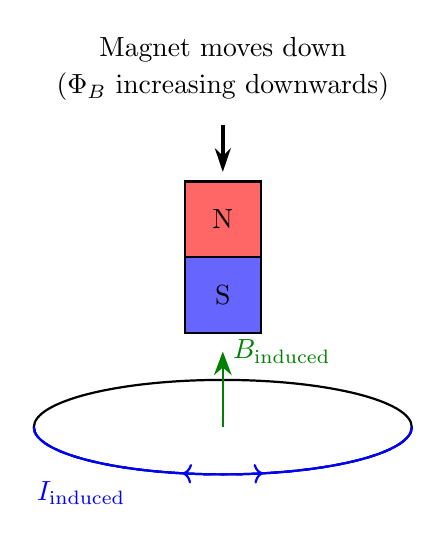
\begin{tikzpicture}[scale=1.2]
    % --- Corrected Lenz's Law Diagram ---
    % Text description
    \node at (0, 4) {Magnet moves down};
    \node at (0, 3.6) {($\Phi_B$ increasing downwards)};
    
    % Velocity vector
    \draw[-{Stealth[length=3mm, width=2mm]}, ultra thick] (0, 3.2) -- (0, 2.7);

    % Bar magnet
    \draw[thick, fill=blue!60] (-0.4, 1.8) rectangle (0.4, 1);
    \node at (0, 1.4) {S};
    \draw[thick, fill=red!60] (-0.4, 2.6) rectangle (0.4, 1.8);
    \node at (0, 2.2) {N};

    % Coil
    \draw[thick] (0,0) ellipse (2cm and 0.5cm);
    
    % Induced B-field (upwards, opposing the change)
    \draw[-{Stealth[length=3mm]}, thick, green!50!black] (0, 0) -- (0, 0.8) node[right] {$B_{\text{induced}}$};
    
    % Induced current (counter-clockwise)
    \begin{scope}[decoration={
        markings,
        mark=at position 0.6 with {\arrow{>}}}
        ]
        % Front part of the coil's current arrow
        \draw[postaction={decorate}, thick, blue] (2,0) arc (0:-180:2cm and 0.5cm);
        % Back part of the coil's current arrow (dashed)
        \draw[postaction={decorate}, thick, blue, dashed] (-2,0) arc (180:360:2cm and 0.5cm);
    \end{scope}
    \node[blue] at (-1.5, -0.7) {$I_{\text{induced}}$};
\end{tikzpicture}
\end{center}

\subsection{Motional EMF}
This is the EMF induced in a conductor moving through a magnetic field.
\begin{itemize}
    \item \textbf{Scenario:} A conductor of length $L$ moves at a constant velocity $\vec{v}$ perpendicular to a uniform magnetic field $\vec{B}$.
    \item \textbf{Equation:}
    $$ \mathcal{E} = BLv $$
\end{itemize}
\begin{center}
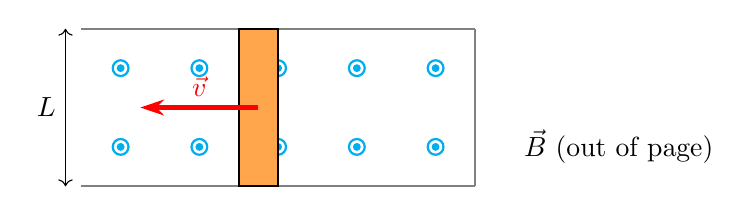
\begin{tikzpicture}
    % Rails
    \draw[thick, gray] (0,2) -- (5,2);
    \draw[thick, gray] (0,0) -- (5,0);
    \draw[thick, gray] (5,0) -- (5,2);
    % B-field
    \foreach \x in {0.5,1.5,...,4.5}
        \foreach \y in {0.5,1.5}
            \draw[cyan, thick] (\x,\y) circle (0.1cm);
    \foreach \x in {0.5,1.5,...,4.5}
        \foreach \y in {0.5,1.5}
            \fill[cyan] (\x,\y) circle (0.05cm);
    \node at (5.5,0.5) [right] {$\vec{B}$ (out of page)};
    % Rod
    \draw[thick, fill=orange!70] (2,0) rectangle (2.5,2);
    % Velocity vector
    \draw[-{Stealth[length=3mm, width=2mm]}, ultra thick, red] (2.25,1) -- (0.75,1) node[midway, above] {$\vec{v}$};
    % Length L
    \draw[<->] (-0.2,0) -- (-0.2,2) node[midway, left] {$L$};
\end{tikzpicture}
\end{center}
\subsection{Energy Conservation \_b}
The energy for the induced current comes from the work done to move the conductor.
\begin{itemize}
    \item The induced current $I$ creates a \textbf{magnetic drag force}, $F_m = ILB$, which opposes the motion.
    \item To maintain constant velocity, an \textbf{external force} $F_{ext} = ILB$ must be applied.
    \item The \textbf{mechanical power} supplied is $P_{\text{mech}} = F_{\text{ext}}v = (ILB)v$.
    \item The \textbf{electrical power} dissipated as heat is $P_{\text{elec}} = I^2R$.
    \item By conservation of energy: $P_{\text{mech}} = P_{\text{elec}}$.
\end{itemize}


\newpage
\section{Original Problem Solutions}

\subsection{Problem 1 (from EMI3.pdf)}

\subsubsection*{Problem Text (EMI3.pdf)}
\begin{quote}
3. The conducting rod shown in the figure has length L and is being pulled along horizontal, frictionless conducting rails at a constant velocity $\vec{v}$. The rails are connected at one end with a metal strip. A uniform magnetic field $\vec{B}$, directed out of the page, fills the region in which the rod moves. Assume that $L=10$ cm, $v=5.0~m/s$ and $B=1.2~T$. What are the (a) magnitude and (b) direction (up or down the page) of the emf induced in the rod? (c) magnitude and (d) direction of the current in the conducting loop? Assume that the resistance of the rod is 0.40 $\Omega$ and that the resistance of the rails and metal strip is negligibly small.
(e) At what rate is thermal energy being generated in the rod?
(f) What external force on the rod is needed to maintain $\vec{v}$?
(g) At what rate does this force do work on the rod?
\end{quote}

\subsubsection*{Solution}
\textbf{Given:} $L = 10 \text{ cm} = 0.10 \text{ m}$, $v = 5.0 \text{ m/s}$, $B = 1.2 \text{ T}$, $R_{\text{rod}} = 0.40 \, \Omega$.

\begin{enumerate}
    \item[(a)] \textbf{Magnitude of the induced EMF}
    $$ \mathcal{E} = BLv = (1.2 \text{ T})(0.10 \text{ m})(5.0 \text{ m/s}) = \mathbf{0.60 \, V} $$

    \item[(b)] \textbf{Direction of the induced EMF}
    Using the Lorentz force on positive charge carriers, $\vec{F} = q(\vec{v} \times \vec{B})$. The velocity $\vec{v}$ is to the left, and the magnetic field $\vec{B}$ is out of the page. The resulting force $\vec{F}$ is downwards. Therefore, the direction of the EMF is \textbf{down}.

    \item[(c)] \textbf{Magnitude of the current}
    $$ I = \frac{\mathcal{E}}{R} = \frac{0.60 \text{ V}}{0.40 \, \Omega} = \mathbf{1.5 \, A} $$
    
    \item[(d)] \textbf{Direction of the current}
    The EMF acts like a battery with the positive terminal at the bottom of the rod. Current flows from positive to negative through the external circuit, resulting in a \textbf{counter-clockwise} loop.

    \item[(e)] \textbf{Rate of thermal energy generation}
    $$ P_{\text{thermal}} = I^2R = (1.5 \text{ A})^2 (0.40 \, \Omega) = \mathbf{0.90 \, W} $$
    
    \item[(f)] \textbf{External force needed}
    The external force must balance the magnetic drag force, $F_m = ILB$.
    $$ F_{\text{ext}} = ILB = (1.5 \text{ A})(0.10 \text{ m})(1.2 \text{ T}) = \mathbf{0.18 \, N} $$
    The force must be applied in the direction of motion, to the \textbf{left}.
    
    \item[(g)] \textbf{Rate at which the external force does work}
    $$ P_{\text{force}} = F_{\text{ext}}v = (0.18 \text{ N})(5.0 \text{ m/s}) = \mathbf{0.90 \, W} $$
    This matches the thermal energy rate, as expected from energy conservation.
\end{enumerate}
\hrule

\subsection{Problem 2 (from EMI1.pdf)}

\subsubsection*{Problem Text (EMI1.pdf)}
\begin{quote}
4. Figure 4 shows a long, straight wire of negligible resistance bent into a V shape, with its two arms making an angle $\alpha$ with each other, and placed horizontally in a vertical uniform magnetic field of strength B. A rod of total mass m, and resistance R per unit length, is placed on the V-shaped conductor, at a distance $x_{0}$ from its vertex A, and perpendicular to the bisector of the angle $\alpha$.
The rod started off with an initial velocity $v_{0}$ in the direction along the bisector, and away from A. The rod is long enough not to fall off the wire during the subsequent motion, and the electrical contact between the two is perfect, while friction between them is negligible.
Show that the rod will stop at $x=\sqrt{x_{0}^{2}+\frac{mv_{0}R}{B^{2}\tan\frac{\alpha}{2}}}.$
\end{quote}

\subsubsection*{Solution}
This problem involves a conductor moving on V-shaped rails, where the length of the conductor in the circuit changes as it moves.

\begin{center}
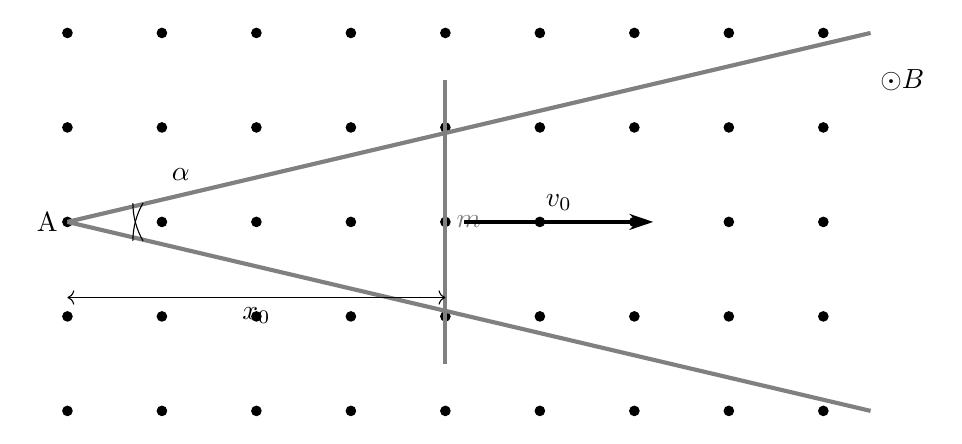
\begin{tikzpicture}[scale=1.2]
    % B-field (dots)
    \foreach \x in {0,1,...,8}
        \foreach \y in {0,1,...,4}
            \filldraw (\x,\y) circle (0.05cm);
    \node at (8.5, 3.5) [right] {$\odot B$};

    % V-shaped wire
    \draw[thick, gray, line width=1.5pt] (0,2) -- (8.5,4);
    \draw[thick, gray, line width=1.5pt] (0,2) -- (8.5,0);
    \node at (0,2) [left] {A};

    % Angle alpha
    \draw (0.8, 2.2) arc (150:180:0.8);
    \draw (0.8, 1.8) arc (210:180:0.8);
    \node at (1.2, 2.5) {$\alpha$};
    
    % Rod
    \draw[thick, gray, fill=white, line width=1.5pt] (4,0.5) -- (4,3.5) node[midway, right] {$m$};
    
    % Initial position and velocity
    \draw[<->] (0,1.2) -- (4,1.2) node[midway, below] {$x_0$};
    \draw[-{Stealth[length=3mm, width=2mm]}, ultra thick] (4.2, 2) -- (6.2, 2) node[midway, above] {$v_0$};
\end{tikzpicture}
\end{center}

\begin{enumerate}
    \item \textbf{Define variables at position $x$:}
    The half-angle of the V-shape is $\frac{\alpha}{2}$.
    \begin{itemize}
        \item The length of the rod in the circuit is $L(x) = 2x \tan(\frac{\alpha}{2})$.
        \item The resistance of the rod is $R_{\text{rod}}(x) = R \cdot L(x) = 2Rx \tan(\frac{\alpha}{2})$.
    \end{itemize}

    \item \textbf{Calculate Induced EMF and Current:}
    \begin{itemize}
        \item Motional EMF: $\mathcal{E} = B L(x) v = B (2x \tan(\frac{\alpha}{2})) v$.
        \item Induced Current: $I = \frac{\mathcal{E}}{R_{\text{rod}}(x)} = \frac{B (2x \tan(\frac{\alpha}{2})) v}{2Rx \tan(\frac{\alpha}{2})} = \frac{Bv}{R}$.
        \item The current $I$ is independent of position $x$.
    \end{itemize}
    
    \item \textbf{Set up the Equation of Motion:}
    The magnetic drag force $F_m$ opposes the motion.
    $$ F_m = I L(x) B = \left(\frac{Bv}{R}\right) \left(2x \tan\left(\frac{\alpha}{2}\right)\right) B = \frac{2B^2v \tan(\frac{\alpha}{2})}{R} x $$
    Using Newton's Second Law ($F_{\text{net}} = ma$):
    $$ m \frac{dv}{dt} = -F_m = -\frac{2B^2 \tan(\frac{\alpha}{2})}{R} x v $$
    
    \item \textbf{Solve the Differential Equation:}
    Use the chain rule: $a = \frac{dv}{dt} = \frac{dv}{dx}\frac{dx}{dt} = v\frac{dv}{dx}$.
    $$ m v\frac{dv}{dx} = -\frac{2B^2 \tan(\frac{\alpha}{2})}{R} x v $$
    Cancel $v$ from both sides and separate variables:
    $$ m \, dv = -\frac{2B^2 \tan(\frac{\alpha}{2})}{R} x \, dx $$
    Integrate from initial state ($v_0, x_0$) to final state ($0, x$):
    $$ \int_{v_0}^{0} m \, dv = \int_{x_0}^{x} -\frac{2B^2 \tan(\frac{\alpha}{2})}{R} x \, dx $$
    $$ m[v]_{v_0}^{0} = -\frac{2B^2 \tan(\frac{\alpha}{2})}{R} \left[\frac{x^2}{2}\right]_{x_0}^{x} $$
    $$ m(0 - v_0) = -\frac{B^2 \tan(\frac{\alpha}{2})}{R} (x^2 - x_0^2) $$
    $$ mv_0 = \frac{B^2 \tan(\frac{\alpha}{2})}{R} (x^2 - x_0^2) $$
    Rearranging to solve for the final position $x$:
    $$ x^2 - x_0^2 = \frac{mv_0 R}{B^2 \tan(\frac{\alpha}{2})} $$
    $$ \mathbf{x = \sqrt{x_0^2 + \frac{mv_0 R}{B^2 \tan(\frac{\alpha}{2})}}} $$
    This matches the required expression.
\end{enumerate}
\hrule

\subsection{Problem 3 (from EMI2.pdf)}

\subsubsection*{Problem Text (EMI2.pdf)}
\begin{quote}
3. (a) A uniform thin wire XY is suspended by two inelastic strings attached to its end. The wire has a mass of 20 g and its resistance is 1.2 $\Omega$. The length of the wire is 50 cm. The wire and the supporting strings are placed in a region where there is a uniform magnetic field of magnitude 40 mT and direction perpendicular to the plane containing the strings and the wire, as shown in Fig. 3. What is the direction and magnitude of the potential difference that must be applied to the wire so that the tension in the strings becomes zero?
\end{quote}

\subsubsection*{Solution}
\textbf{Given:} $m = 20 \text{ g} = 0.020 \text{ kg}$, $R = 1.2 \, \Omega$, $L = 50 \text{ cm} = 0.50 \text{ m}$, $B = 40 \text{ mT} = 0.040 \text{ T}$.

\begin{center}
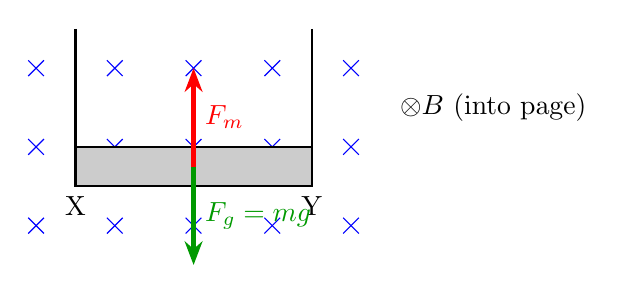
\begin{tikzpicture}
    % B-field (crosses)
    \foreach \x in {0.5,1.5,...,4.5}
        \foreach \y in {-0.5,0.5,1.5}
            \draw[blue] (\x-0.1, \y-0.1) -- (\x+0.1, \y+0.1);
    \foreach \x in {0.5,1.5,...,4.5}
        \foreach \y in {-0.5,0.5,1.5}
            \draw[blue] (\x-0.1, \y+0.1) -- (\x+0.1, \y-0.1);
    \node at (5, 1) [right] {$\otimes B$ (into page)};

    % Suspended Wire
    \draw[thick] (1,2) -- (1,0.5);
    \draw[thick] (4,2) -- (4,0.5);
    \draw[thick, fill=gray!40] (1,0.5) rectangle (4,0);
    \node at (1, -0.25) {X};
    \node at (4, -0.25) {Y};
    
    % Forces
    \draw[-{Stealth[length=3mm]}, ultra thick, red] (2.5,0.25) -- (2.5,1.5) node[midway, right] {$F_m$};
    \draw[-{Stealth[length=3mm]}, ultra thick, green!60!black] (2.5,0.25) -- (2.5,-1) node[midway, right] {$F_g = mg$};
\end{tikzpicture}
\end{center}

\begin{enumerate}
    \item \textbf{Condition for Zero Tension:}
    For zero tension, the upward magnetic force ($F_m$) must balance the downward gravitational force ($F_g$).
    $$ F_m = F_g $$
    
    \item \textbf{Calculate the Required Current:}
    $$ F_g = mg = (0.020 \text{ kg})(9.8 \text{ m/s}^2) = 0.196 \text{ N} $$
    $$ F_m = ILB \implies I = \frac{mg}{LB} = \frac{0.196 \text{ N}}{(0.50 \text{ m})(0.040 \text{ T})} = \mathbf{9.8 \, A} $$

    \item \textbf{Determine the Potential Difference:}
    Using Ohm's Law:
    $$ V = IR = (9.8 \text{ A})(1.2 \, \Omega) = \mathbf{11.76 \, V} \approx 12 \, \text{V} $$
    
    \item \textbf{Determine the Direction:}
    To get an upward force ($\vec{F}$) with a magnetic field ($\vec{B}$) into the page, the Right-Hand Rule ($\vec{F} = I(\vec{L} \times \vec{B})$) dictates that the current ($I$) must flow from left to right. Therefore, current flows from \textbf{X to Y}, meaning \textbf{X must be at a higher potential than Y}.
\end{enumerate}
\hrule

\subsection{Problem 4 (from EMI4.pdf)}

\subsubsection*{Problem Text (EMI4.pdf)}
\begin{quote}
3. One end of a thin conducting rod of length l is pivoted to a fixed point. The rod has a resistance of R and its two ends of the rod are connected to a resistor with resistance $R_{0}$. The rod is rotating with a constant angular velocity in a uniform magnetic field of flux density B. This direction of magnetic field is normal to the plane of rotation of the rod.
(a) What is the emf induced in the rod?
(b) Determine the electric power developed in the resistor.
(c) Describe, with evidence, the origin of the electric power developed in the resistor.
\end{quote}

\subsubsection*{Solution}
A conducting rod of length $l$ and resistance $R$ rotates at a constant angular velocity $\omega$ in a uniform magnetic field $B$. It is connected to an external resistor $R_0$.

\begin{center}
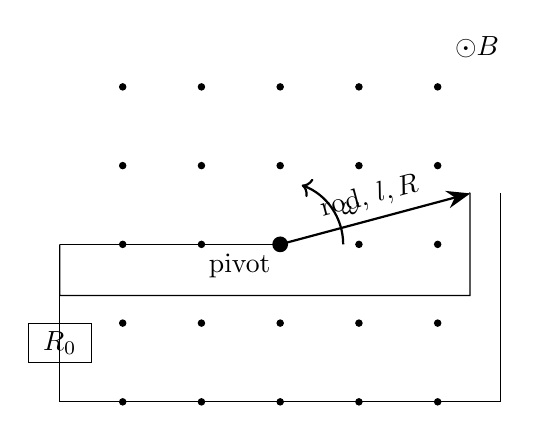
\begin{tikzpicture}
    % B-field (dots)
    \foreach \x in {-2,-1,...,2}
        \foreach \y in {-2,-1,...,2}
            \filldraw (\x,\y) circle (0.04cm);
    \node at (2.5, 2.5) {$\odot B$};

    % Rotating Rod
    \draw[thick, -{Stealth[length=3mm]}] (0,0) -- (15:2.5cm) node[midway, above, sloped] {rod, $l, R$};
    \fill (0,0) circle (0.1cm) node[below left] {pivot};
    \draw[->, thick] (0.8,0) arc (0:70:0.8cm) node[midway, right] {$\omega$};

    % External Circuit
    \draw (0,0) -- (-2.8, 0);
    \draw (15:2.5cm) -- (2.41, 0.65) -- (2.41, -0.65) -- (-2.8, -0.65) -- (-2.8, 0);
    % Resistor R0
    \draw (-2.8, -0.65) -- (-2.8, -1);
    \draw (-3.2, -1) rectangle (-2.4, -1.5);
    \node at (-2.8, -1.25) {$R_0$};
    \draw (-2.8, -1.5) -- (-2.8, -2);
    \draw (-2.8, -2) -- (-2.8, -0.65) [xshift=5.6cm];
    \draw (-2.8, -2) -- (2.8, -2) -- (2.8, 0.65);
\end{tikzpicture}
\end{center}

\begin{enumerate}
    \item[(a)] \textbf{What is the emf induced in the rod?}
    A small segment $dr$ at distance $r$ from the pivot has velocity $v = \omega r$. The EMF across it is $d\mathcal{E} = Bv \, dr = B(\omega r) \, dr$.
    To find the total EMF, we integrate from $r=0$ to $r=l$:
    $$ \mathcal{E} = \int_{0}^{l} B\omega r \, dr = B\omega \left[ \frac{r^2}{2} \right]_{0}^{l} $$
    $$ \mathcal{E} = \frac{1}{2} B\omega l^2 $$
    
    \item[(b)] \textbf{Determine the electric power developed in the resistor.}
    Total resistance of the series circuit is $R_{\text{total}} = R + R_0$.
    The current is $I = \frac{\mathcal{E}}{R_{\text{total}}} = \frac{B\omega l^2}{2(R + R_0)}$.
    The power in the external resistor $R_0$ is $P_{R_0} = I^2 R_0$:
    $$ P_{R_0} = \left( \frac{B\omega l^2}{2(R + R_0)} \right)^2 R_0 = \frac{B^2\omega^2 l^4 R_0}{4(R + R_0)^2} $$
    
    \item[(c)] \textbf{Describe, with evidence, the origin of the electric power.}
    \textbf{Origin:} The electric power originates from the \textbf{mechanical work} done by an external torque to keep the rod rotating at a constant angular velocity against the magnetic drag torque.

    \textbf{Evidence (Energy Conservation):}
    \begin{itemize}
        \item The current $I$ creates a magnetic force $dF_m = I B dr$ on each segment $dr$.
        \item This force creates a drag torque $d\tau_m = r \, dF_m = rIB \, dr$.
        \item The total magnetic drag torque is:
        $$ \tau_m = \int_{0}^{l} rIB \, dr = IB \left[ \frac{r^2}{2} \right]_{0}^{l} = \frac{1}{2} IBl^2 $$
        \item To maintain constant $\omega$, an external torque $\tau_{\text{ext}} = \tau_m$ must be applied.
        \item The mechanical power supplied is $P_{\text{mech}} = \tau_{\text{ext}} \omega = (\frac{1}{2} IBl^2) \omega$.
        \item The total electrical power dissipated in the circuit is $P_{\text{elec}} = I^2 R_{\text{total}} = I^2(R+R_0)$.
        \item Since $I = \frac{\mathcal{E}}{R+R_0}$ and $\mathcal{E} = \frac{1}{2}B\omega l^2$, we can write $I(R+R_0) = \mathcal{E}$.
        \item Let's check if $P_{\text{mech}} = P_{\text{elec}}$:
        $$ P_{\text{mech}} = \omega \left( \frac{1}{2}Bl^2 \right) I = \mathcal{E}I $$
        $$ P_{\text{elec}} = I^2(R+R_0) = I \cdot (I(R+R_0)) = I\mathcal{E} $$
        Since $P_{\text{mech}} = \mathcal{E}I$ and $P_{\text{elec}} = \mathcal{E}I$, the mechanical power supplied by the external torque is equal to the total electrical power dissipated in the circuit. This confirms the origin of the power.
    \end{itemize}
\end{enumerate}

\newpage
\section{New Problem Solutions}

\section{New Problem 1: Rod Sliding on an Inclined Plane}
This problem combines motional EMF with mechanics, similar to the setup in `EMI3.pdf` but adding the element of gravity.

\subsection{Question}
A conducting rod of mass $m = 50 \text{ g}$ and resistance $R = 0.25 \, \Omega$ is placed on two frictionless, parallel conducting rails inclined at an angle $\theta = 30^\circ$ to the horizontal. The rails have negligible resistance and are connected at the bottom by a wire. The entire setup is in a uniform vertical magnetic field of magnitude $B = 0.50 \text{ T}$, as shown in the diagram. The rod is released from rest.

\begin{center}
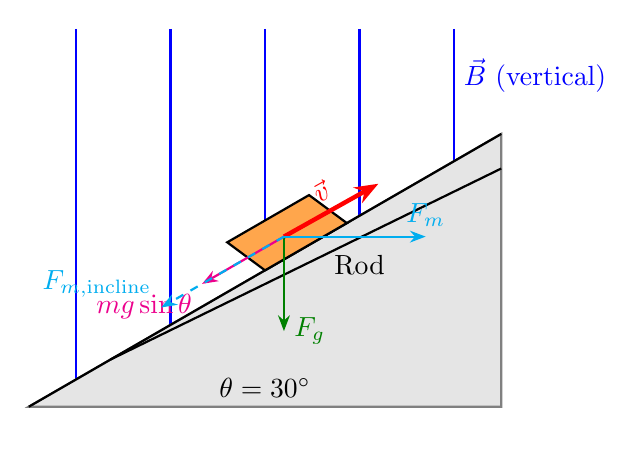
\begin{tikzpicture}[scale=1.2, rotate=0]
    % Draw B field vectors (vertical)
    \foreach \x in {0.5, 1.5, 2.5, 3.5, 4.5} {
        \draw[-{Stealth[length=2mm]}, thick, blue] (\x, 4) -- (\x, 0) node[below] {};
    }
    \node[blue, right] at (4.5, 3.5) {$\vec{B}$ (vertical)};
    
    % Draw inclined plane
    \draw[thick, gray, fill=gray!20] (0,0) -- (5,0) -- (5, 2.887) -- cycle; % 5*tan(30) = 2.887
    
    % Draw rails on the incline
    \draw[thick] (0.866, 0.5) -- (5, 2.887 - 0.5*1.732 + 0.5); % Rail 1
    \draw[thick] (0,0) -- (5, 2.887); % Rail 2
    \node at (2.5, 0.2) {$\theta=30^\circ$};
    
    % Draw conducting rod
    \draw[thick, fill=orange!70] (2.5, 1.4435) -- (3.366, 1.9435) -- (2.966, 2.24) -- (2.1, 1.74) -- cycle;
    \node at (3.5, 1.5) {Rod};
    
    % Velocity vector
    \draw[-{Stealth[length=3mm]}, ultra thick, red] (2.7, 1.8) -- (3.7, 2.36) node[midway, above, sloped] {$\vec{v}$};
    
    % Force vectors on the rod (as a point for clarity)
    \coordinate (rodcenter) at (2.7, 1.8);
    \draw[-{Stealth[length=2mm]}, thick, green!50!black] (rodcenter) --++ (0,-1) node[right]{$F_g$};
    \draw[-{Stealth[length=2mm]}, thick, magenta] (rodcenter) --++ (-1.732/2, -1/2) node[below left]{$mg\sin\theta$};
    \draw[-{Stealth[length=2mm]}, thick, cyan] (rodcenter) --++ (1.5,0) node[above]{$F_m$};
    \draw[-{Stealth[length=2mm]}, thick, cyan, dashed] (rodcenter) --++ (-1.5*0.866, -1.5*0.5) node[above left]{$F_{m, \text{incline}}$};
\end{tikzpicture}
\end{center}

\begin{enumerate}
    \item[(a)] Find the terminal velocity ($v_t$) of the rod as it slides down the incline.
    \item[(b)] What is the magnitude of the induced current at this terminal velocity?
    \item[(c)] Show that the rate of electrical energy dissipation is equal to the rate of gravitational potential energy loss at terminal velocity.
\end{enumerate}

\subsection{Explanation and Solution}
\begin{enumerate}
    \item[(a)] \textbf{Finding the Terminal Velocity}\\
    The magnetic flux through the loop is $\Phi_B = \vec{B} \cdot \vec{A} = B A \cos\theta$, where $A=Lx$ is the area of the loop and $x$ is the distance the rod has slid.
    The induced EMF is $|\mathcal{E}| = \frac{d\Phi_B}{dt} = \frac{d}{dt}(BLx \cos\theta) = BLv \cos\theta$.
    The induced current is $I = \frac{\mathcal{E}}{R} = \frac{BLv \cos\theta}{R}$.
    The magnetic force on the rod is $\vec{F}_m = I(\vec{L} \times \vec{B})$. This force is horizontal with magnitude $F_m = ILB$. Its component opposing motion along the incline is $F_{m, \text{incline}} = F_m \cos\theta = (ILB)\cos\theta$.
    At terminal velocity ($v_t$), the net force is zero, so the gravitational component pulling the rod down is balanced by the magnetic component pushing it up the incline.
    $$ mg \sin\theta = F_{m, \text{incline}} $$
    $$ mg \sin\theta = \left(\frac{BLv_t \cos\theta}{R}\right)LB\cos\theta = \frac{B^2 L^2 v_t \cos^2\theta}{R} $$
    Solving for $v_t$ and assuming a standard rail width $L=1.0 \text{ m}$:
    $$ v_t = \frac{mgR \sin\theta}{B^2 L^2 \cos^2\theta} = \frac{(0.050)(9.8)(0.25)\sin(30^\circ)}{(0.50)^2 (1.0)^2 \cos^2(30^\circ)} = \mathbf{0.327 \, m/s} $$

    \item[(b)] \textbf{Current at Terminal Velocity}\\
    Substitute $v_t$ back into the equation for current:
    $$ I = \frac{BLv_t \cos\theta}{R} = \frac{(0.50)(1.0)(0.327)\cos(30^\circ)}{0.25} = \mathbf{0.566 \, A} $$

    \item[(c)] \textbf{Energy Conservation}\\
    Rate of electrical energy dissipation (power):
    $$ P_{elec} = I^2R = (0.566)^2(0.25) = \mathbf{0.080 \, W} $$
    Rate of gravitational potential energy loss:
    $$ P_{grav} = (mg \sin\theta) v_t = (0.050)(9.8)\sin(30^\circ)(0.327) = \mathbf{0.080 \, W} $$
    Since $P_{elec} = P_{grav}$, energy is conserved.
\end{enumerate}
\hrule

\section{New Problem 2: The Levitating Square Coil}
This problem tests the concept of magnetic force in a non-uniform field.

\subsection{Question}
A square coil with side length $l = 10 \text{ cm}$, $N=50$ turns, and mass $m = 100 \text{ g}$ is positioned in a non-uniform magnetic field. The magnetic field is horizontal but its magnitude increases vertically upwards, given by $\vec{B}(y) = (ky) \hat{x}$, where $k = 2.0 \text{ T/m}$. The coil is in the y-z plane. What is the magnitude and direction of the current $I$ required for the coil to levitate?

\begin{center}
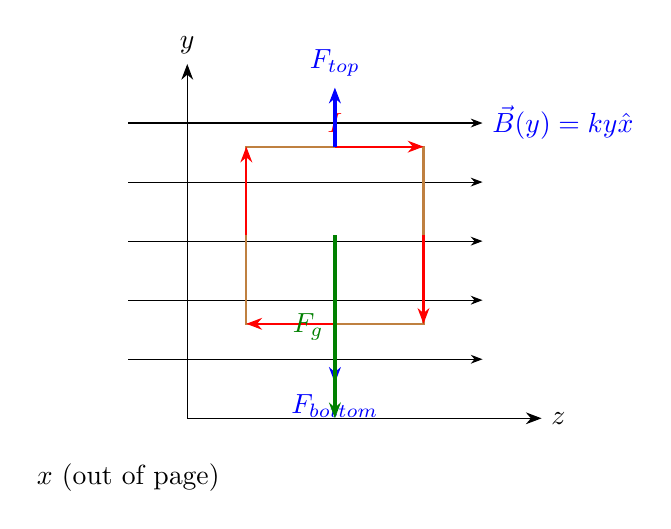
\begin{tikzpicture}[scale=1.5]
    % Y and Z axes
    \draw[-{Stealth[length=2mm]}] (0,0) -- (0,3) node[above] {$y$};
    \draw[-{Stealth[length=2mm]}] (0,0) -- (3,0) node[right] {$z$};
    \node at (-0.5,-0.5) {$x$ (out of page)};

    % Magnetic field lines (horizontal, increasing density upwards)
    \foreach \y in {0.5, 1, 1.5, 2, 2.5} {
        \draw[-{Stealth[length=1.5mm]}] (-0.5, \y) -- (2.5, \y);
    }
    \node[blue, right] at (2.5, 2.5) {$\vec{B}(y) = ky\hat{x}$};

    % Square coil
    \draw[thick, brown] (0.5, 0.8) rectangle (2, 2.3);
    
    % Current direction arrows
    \draw[-{Stealth[length=2mm]}, red, thick] (0.5, 1.55) -- (0.5, 2.3); % Left side up
    \draw[-{Stealth[length=2mm]}, red, thick] (1.25, 2.3) -- (2, 2.3); % Top side right (+z)
    \draw[-{Stealth[length=2mm]}, red, thick] (2, 1.55) -- (2, 0.8); % Right side down
    \draw[-{Stealth[length=2mm]}, red, thick] (1.25, 0.8) -- (0.5, 0.8); % Bottom side left (-z)
    \node[red] at (1.25, 2.5) {$I$};
    
    % Force vectors
    \draw[-{Stealth[length=2mm]}, ultra thick, blue] (1.25, 0.8) -- (1.25, 0.3) node[below] {$F_{bottom}$};
    \draw[-{Stealth[length=2mm]}, ultra thick, blue] (1.25, 2.3) -- (1.25, 2.8) node[above] {$F_{top}$};
    \draw[-{Stealth[length=2mm]}, ultra thick, green!50!black] (1.25, 1.55) -- (1.25, 0) node[midway, left] {$F_g$};
\end{tikzpicture}
\end{center}

\subsection{Explanation and Solution}
The forces on the vertical sides of the coil are in the $\pm \hat{z}$ direction and cancel each other out. We only need to consider the horizontal sides.
\begin{itemize}
    \item \textbf{Bottom Side (at y):} The force is downwards. $\vec{F}_{bottom} = I (l(-\hat{z})) \times (ky \hat{x}) = -Ikly (\hat{z} \times \hat{x}) = -Ikly \hat{y}$.
    \item \textbf{Top Side (at y+l):} The force is upwards. $\vec{F}_{top} = I (l(\hat{z})) \times (k(y+l) \hat{x}) = Ikl(y+l) (\hat{z} \times \hat{x}) = Ikl(y+l) \hat{y}$.
\end{itemize}
The net magnetic force for $N$ turns is:
$$ \vec{F}_{net, m} = N(\vec{F}_{top} + \vec{F}_{bottom}) = N(Ikl(y+l) - Ikly)\hat{y} = NIkl^2 \hat{y} $$
For levitation, this must balance gravity ($F_g = mg$):
$$ NIkl^2 = mg $$
Solving for the current $I$:
$$ I = \frac{mg}{Nkl^2} = \frac{(0.100 \text{ kg})(9.8 \text{ m/s}^2)}{(50)(2.0 \text{ T/m})(0.10 \text{ m})^2} = \mathbf{0.98 \, A} $$
The direction must be as shown in the diagram to produce an upward force on the top wire.

\hrule

\section{New Problem 3: The Faraday Disk}
This problem explores motional EMF in a solid rotating disk.

\subsection{Question}
A copper disk of radius $a = 20 \text{ cm}$ rotates at $\omega = 300 \text{ rad/s}$ in a uniform magnetic field $B = 1.5 \text{ T}$ perpendicular to its plane. A circuit is formed using sliding contacts at the center and the rim, connected to a resistor $R_0 = 2.0 \, \Omega$. The disk's resistance is negligible.

\begin{center}
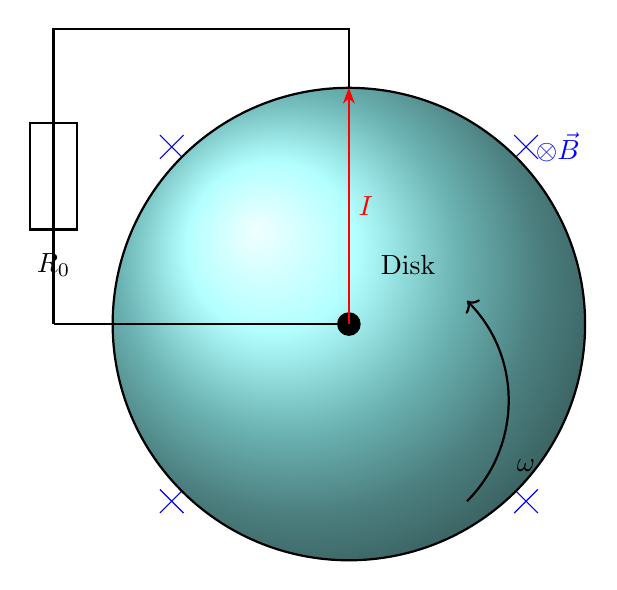
\begin{tikzpicture}[scale=1.5]
    % B-field (into page)
    \foreach \x in {-1.5, -0.5, 0.5, 1.5}
        \foreach \y in {-1.5, -0.5, 0.5, 1.5} {
            \draw[blue] (\x-0.1, \y-0.1) -- (\x+0.1, \y+0.1);
            \draw[blue] (\x-0.1, \y+0.1) -- (\x+0.1, \y-0.1);
        }
    \node[blue, right] at (1.5, 1.5) {$\otimes \vec{B}$};

    % Disk
    \shade[ball color=cyan!40] (0,0) circle (2cm);
    \draw[thick] (0,0) circle (2cm);
    \fill (0,0) circle (0.1cm);
    \node at (0.5, 0.5) {Disk};
    
    % Rotation
    \draw[->, thick] (1, -1.5) arc (-45:45:1.2cm);
    \node at (1.5, -1.2) {$\omega$};
    
    % External circuit
    \draw[thick] (0,0) -- (-2.5, 0); % Axle contact
    \draw[thick] (0, 2) -- (0, 2.5) -- (-2.5, 2.5) -- (-2.5, 0); % Rim contact
    \draw[thick] (-2.7, 0.8) rectangle (-2.3, 1.7); % Resistor
    \node at (-2.5, 0.5) {$R_0$};
    
    % Current flow
    \draw[-{Stealth[length=2mm]}, red, thick] (0,0) -- (0,2);
    \node[red, right] at (0,1) {$I$};
\end{tikzpicture}
\end{center}

\begin{enumerate}
    \item[(a)] What is the magnitude of the EMF induced between the center and the rim?
    \item[(b)] What is the current that flows through the external resistor?
    \item[(c)] Calculate the external torque required to keep the disk rotating.
\end{enumerate}

\subsection{Explanation and Solution}
\begin{enumerate}
    \item[(a)] \textbf{Induced EMF}\\
    We integrate the motional EMF $d\mathcal{E} = Bv\,dr = B(\omega r)dr$ from the center to the rim.
    $$ \mathcal{E} = \int_{0}^{a} B\omega r \, dr = B\omega \left[ \frac{r^2}{2} \right]_{0}^{a} = \frac{1}{2} B\omega a^2 $$
    $$ \mathcal{E} = \frac{1}{2} (1.5)(300)(0.20)^2 = \mathbf{9.0 \, V} $$
    
    \item[(b)] \textbf{Current}\\
    Using Ohm's law with the external resistor:
    $$ I = \frac{\mathcal{E}}{R_0} = \frac{9.0 \text{ V}}{2.0 \, \Omega} = \mathbf{4.5 \, A} $$
    
    \item[(c)] \textbf{External Torque}\\
    The current $I$ flowing radially in the magnetic field creates a drag torque. We integrate the torque element $d\tau_m = r \, dF_m = r(IB\,dr)$ from center to rim.
    $$ \tau_m = \int_{0}^{a} rIB \, dr = IB \left[ \frac{r^2}{2} \right]_{0}^{a} = \frac{1}{2} I B a^2 $$
    The external torque must balance this drag torque:
    $$ \tau_{ext} = \frac{1}{2} (4.5 \text{ A})(1.5 \text{ T})(0.20 \text{ m})^2 = \mathbf{0.135 \, N \cdot m} $$
\end{enumerate}
\hrule

\section{New Problem 4: The Expanding Loop}
This problem involves a changing loop area and the application of Faraday's Law.

\subsection{Question}
A square conducting loop of initial side length $x_0$ and resistance $R$ is being pulled outwards from two opposite sides. Each side moves with a constant velocity $v_0$. The loop remains in a uniform magnetic field $B$ perpendicular to its plane.

\begin{center}
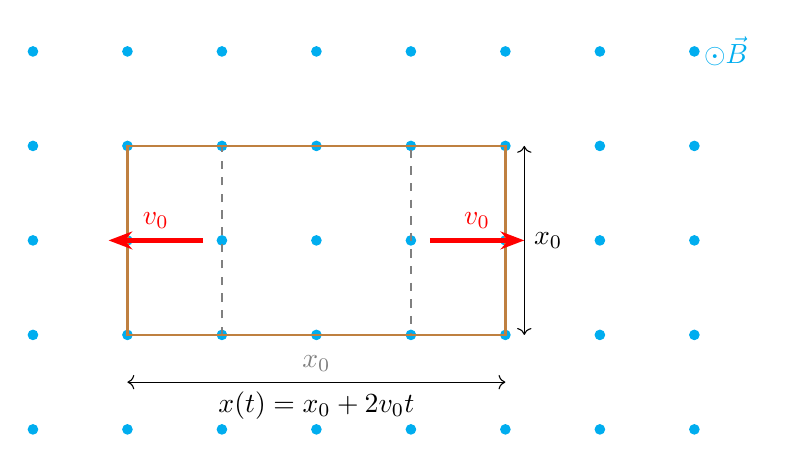
\begin{tikzpicture}[scale=1.2]
    % B-field (dots)
    \foreach \x in {-2,-1,...,5}
        \foreach \y in {-1,...,3}
            \filldraw[cyan] (\x,\y) circle (0.05cm);
    \node[cyan, right] at (5, 3) {$\odot \vec{B}$};

    % Initial loop (dashed)
    \draw[thick, dashed, gray] (0,0) rectangle (2,2);
    \node[gray] at (1,-0.3) {$x_0$};
    
    % Expanding loop at time t
    \draw[thick, brown] (-1,0) rectangle (3,2);
    
    % Velocity vectors
    \draw[-{Stealth[length=3mm]}, ultra thick, red] (-0.2, 1) -- (-1.2, 1) node[midway, above] {$v_0$};
    \draw[-{Stealth[length=3mm]}, ultra thick, red] (2.2, 1) -- (3.2, 1) node[midway, above] {$v_0$};
    
    % Dimensions
    \draw[<->] (-1, -0.5) -- (3, -0.5) node[midway, below] {$x(t) = x_0 + 2v_0t$};
    \draw[<->] (3.2, 0) -- (3.2, 2) node[midway, right] {$x_0$};
\end{tikzpicture}
\end{center}

\begin{enumerate}
    \item[(a)] Find an expression for the induced EMF in the loop as a function of time.
    \item[(b)] Find an expression for the magnitude of the external force required to pull one side of the loop at the constant velocity $v_0$.
\end{enumerate}

\subsection{Explanation and Solution}
\begin{enumerate}
    \item[(a)] \textbf{Induced EMF}\\
    The area of the loop at time $t$ is a rectangle with sides $x_0$ and $(x_0+2v_0t)$.
    $$ A(t) = x_0 (x_0 + 2v_0 t) $$
    The magnetic flux is $\Phi_B = B \cdot A(t) = Bx_0(x_0 + 2v_0 t)$.
    Using Faraday's Law, the magnitude of the EMF is the rate of change of flux:
    $$ |\mathcal{E}| = \left|-\frac{d\Phi_B}{dt}\right| = \left|-\frac{d}{dt} [Bx_0^2 + 2Bx_0v_0 t]\right| $$
    $$ |\mathcal{E}| = 2Bx_0v_0 $$
    The induced EMF is constant.
    
    \item[(b)] \textbf{External Force}\\
    The induced current is $I = \frac{|\mathcal{E}|}{R} = \frac{2Bx_0v_0}{R}$.
    This current flows through the side being pulled (which has length $x_0$), creating a magnetic drag force that opposes the motion.
    $$ F_m = I L B = \left(\frac{2Bx_0v_0}{R}\right) x_0 B = \frac{2B^2x_0^2v_0}{R} $$
    To maintain a constant velocity, the external force must be equal in magnitude to this drag force.
    $$ F_{ext} = \frac{2B^2x_0^2v_0}{R} $$
\end{enumerate}


\end{document}